% abtex2-modelo-artigo.tex, v-1.9.2 laurocesar
% Copyright 2012-2014 by abnTeX2 group at http://abntex2.googlecode.com/ 
%

% ------------------------------------------------------------------------
% ------------------------------------------------------------------------
% abnTeX2: Modelo de Artigo Acadêmico em conformidade com
% ABNT NBR 6022:2003: Informação e documentação - Artigo em publicação 
% periódica científica impressa - Apresentação
% ------------------------------------------------------------------------
% ------------------------------------------------------------------------

\documentclass[
    % -- opções da classe memoir --
    article,            % indica que é um artigo acadêmico
    11pt,               % tamanho da fonte
    oneside,            % para impressão apenas no verso. Oposto a twoside
    a4paper,            % tamanho do papel. 
    % -- opções da classe abntex2 --
    %chapter=TITLE,     % títulos de capítulos convertidos em letras maiúsculas
    %section=TITLE,     % títulos de seções convertidos em letras maiúsculas
    %subsection=TITLE,  % títulos de subseções convertidos em letras maiúsculas
    %subsubsection=TITLE % títulos de subsubseções convertidos em letras maiúsculas
    % -- opções do pacote babel --
    english,            % idioma adicional para hifenização
    brazil,             % o último idioma é o principal do documento
    sumario=tradicional
    ]{abntex2}


% ---
% PACOTES
% ---

% ---
% Pacotes fundamentais 
% ---
\usepackage{lmodern}            % Usa a fonte Latin Modern
\usepackage[T1]{fontenc}        % Selecao de codigos de fonte.
\usepackage[utf8]{inputenc}     % Codificacao do documento (conversão automática dos acentos)
\usepackage{indentfirst}        % Indenta o primeiro parágrafo de cada seção.
\usepackage{nomencl}            % Lista de simbolos
\usepackage{color}              % Controle das cores
\usepackage{graphicx}           % Inclusão de gráficos
\usepackage{microtype}          % para melhorias de justificação
\usepackage{graphicx}			% Inclusão de gráficos
% ---
        
% ---
% Pacotes adicionais, usados apenas no âmbito do Modelo Canônico do abnteX2
% ---
\usepackage{lipsum}             % para geração de dummy text
% ---
        
% ---
% Pacotes de citações
% ---
\usepackage[brazilian,hyperpageref]{backref}     % Paginas com as citações na bibl
\usepackage[alf]{abntex2cite}   % Citações padrão ABNT
% ---

% ---
% Configurações do pacote backref
% Usado sem a opção hyperpageref de backref
\renewcommand{\backrefpagesname}{Citado na(s) página(s):~}
% Texto padrão antes do número das páginas
\renewcommand{\backref}{}
% Define os textos da citação
\renewcommand*{\backrefalt}[4]{
    \ifcase #1 %
        Nenhuma citação no texto.%
    \or
        Citado na página #2.%
    \else
        Citado #1 vezes nas páginas #2.%
    \fi}%
% ---

% ---
% Informações de dados para CAPA e FOLHA DE ROSTO
% ---
\titulo{Desenvolvimento de aplicações com JavaScript}
\autor{Rodrigo Cichetto Monteiro \\ UNIP - Universidade Paulista}
% \local{Araraquara - SP, Brasil}
\data{26 de agosto de 2018, v-1.0.0}
% ---

% ---
% Configurações de aparência do PDF final

% alterando o aspecto da cor azul
\definecolor{blue}{RGB}{41,5,195}

% informações do PDF
\makeatletter
\hypersetup{
        %pagebackref=true,
        pdftitle={\@title}, 
        pdfauthor={\@author},
        pdfsubject={Modelo de artigo científico com abnTeX2},
        pdfcreator={LaTeX with abnTeX2},
        pdfkeywords={abnt}{latex}{abntex}{abntex2}{atigo científico}, 
        colorlinks=true,            % false: boxed links; true: colored links
        linkcolor=blue,             % color of internal links
        citecolor=blue,             % color of links to bibliography
        filecolor=magenta,              % color of file links
        urlcolor=blue,
        bookmarksdepth=4
}
\makeatother
% --- 

% ---
% compila o indice
% ---
\makeindex
% ---

% --- 
% CONFIGURAÇÃO DE FIGURAS
% --- 
\graphicspath{ {imagens/} }

% ---
% Altera as margens padrões
% ---
\setlrmarginsandblock{3cm}{3cm}{*}
\setulmarginsandblock{3cm}{3cm}{*}
\checkandfixthelayout
% ---

% --- 
% Espaçamentos entre linhas e parágrafos 
% --- 

% O tamanho do parágrafo é dado por:
\setlength{\parindent}{1.3cm}

% Controle do espaçamento entre um parágrafo e outro:
\setlength{\parskip}{0.2cm}  % tente também \onelineskip

% Espaçamento simples
\SingleSpacing

% ----
% Início do documento
% ----
\begin{document}

% Retira espaço extra obsoleto entre as frases.
\frenchspacing 

% ----------------------------------------------------------
% ELEMENTOS PRÉ-TEXTUAIS
% ----------------------------------------------------------

%---
%
% Se desejar escrever o artigo em duas colunas, descomente a linha abaixo
% e a linha com o texto ``FIM DE ARTIGO EM DUAS COLUNAS''.
% \twocolumn[           % INICIO DE ARTIGO EM DUAS COLUNAS
%
%---
% página de titulo
\maketitle

% resumo em português
\begin{resumoumacoluna}
Fazendo parte das três principais tecnologias que movem a internet, sendo elas HTML, CSS e claro o JavaScript, a linguagem também conhecida pelo acrônimo JS não é mais voltada somente para desenvolvedores front-end. Nos últimos tempos a linguagem ganhou muita importância em quaisquer cenários, e vem sendo utilizada em sites, aplicações, mobile, servidores, automação de testes, automação de tarefas, internet das coisas, entre outros. Este trabalho tem como principal objetivo apresentar ao leitor uma arquitetura que tem como base a construção de aplicações utilizando a linguagem JavaScript, mostrando os frameworks mais recentes e mais famosos. Mas lembre-se com grandes poderes vem grandes responsabilidades.
 
 \vspace{\onelineskip}
 
 \noindent
 \textbf{Palavras-chaves}: aplicações, javascript, arquitetura
\end{resumoumacoluna}

% ]                 % FIM DE ARTIGO EM DUAS COLUNAS
% ---

% ----------------------------------------------------------
% ELEMENTOS TEXTUAIS
% ----------------------------------------------------------
\textual

% ----------------------------------------------------------
% Introdução
% ----------------------------------------------------------
\section*{Introdução}
\addcontentsline{toc}{section}{Introdução}

Implementada com foco no desenvolvimento web para o lado do
cliente, a linguagem criada por Brendan Eich enquanto trabalhou na Netscape se tornou
uma das linguagens mais populares da atualidade.

Nos últimos anos a linguagem JavaScript ganhou maior importância, com o
surgimento de bibliotecas e frameworks que possibilitaram o desenvolvimento de não
somente web sites mas também aplicativos, single page applications, programas desktop,
progressive web apps e muito mais. Sendo alguns deles Angular, React, Vue, jQuery e
Node.js.

Se existe alguma linguagem que evoluiu nos últimos tempos, essa linguagem é o JavaScript. Em busca de  sua identidade a linguagem foi a única que conseguiu se enraizar nos navegadores, e atualmente também passou a se empoderar dos servidores de alta performance através do Node.js.

Sempre que vamos programar web utilizamos uma ou mais linguagens de programação, PHP, Java, Python para fazer o back-end e utilizamos o HTML com CSS e o JavaScript para o front-end, além de um banco de dados para armazenar as informações.

É bem atraente a possibilidade de usar apenas uma linguagem em todo o desenvolvimento, ganhando não só reaproveitamento de recursos humanos como de código, sendo assim possível criar códigos que podem ser executados em qualquer plataforma que interprete JavaScript.

% ----------------------------------------------------------
% Seção de explicações
% ----------------------------------------------------------
\section{MEAN Stack - A arquitetura}

É possível resolver grande parte dos problemas utilizando o princípo de que um cliente consome as informações de um serviço que fica disponível através de um servidor e persiste os dados em um banco de dados.

Das iniciais das ferramentas MongoDB, Express, Angular e Node.js, MEAN é o nome dado quando integramos todas essas ferramentas para desenvolver uma aplicação. Sendo que todas utilizam como linguagem o JavaScript, possibilitando que um programador da linguagem tenha maior facilidade para trabalhar em todas as partes da aplicação, seja front-end, back-end ou banco de dados.

A onipresença da linguagem JavaScript ajuda na integração da equipe front-end e back-end, melhorando até mesmo a produtividade.

Não devemos focar nas ferramentas em si, mas sim em suas funções que fazem a engrenagem girar, como vemos na Figura \ref{fig:MEANStackFlow}, dividimos a arquitetura em 3 partes, sendo elas o cliente, servidor e banco de dados. Perceba que podemos trocar as peças, desde que a estrutura se mantenha a mesma tudo irá funcionar.

\begin{figure}[h]
	\centering

	\caption{\textit{MEAN Stack} - Fluxo das ferramentas que integram o MEAN} \label{fig:MEANStackFlow}
    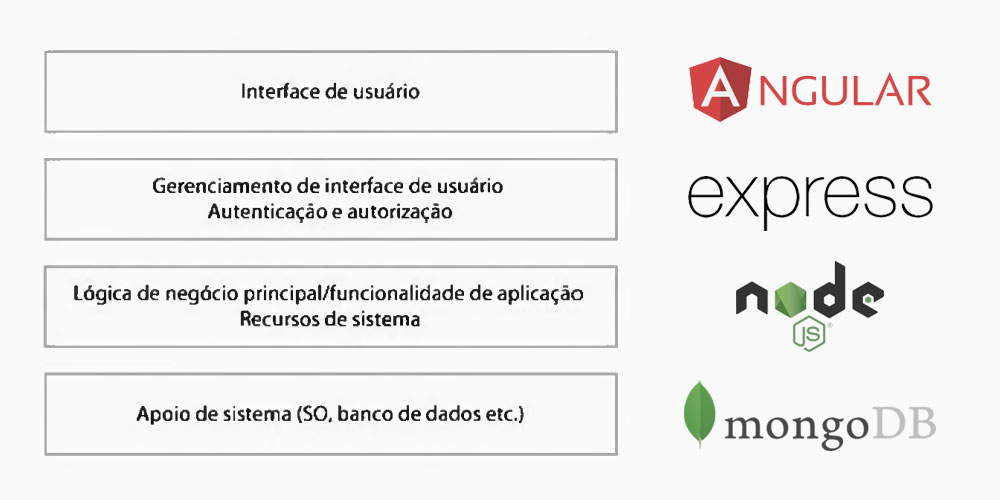
\includegraphics[scale=0.4]{mean-stack-flow} \\
    Fonte: {orangemantra \url{https://www.orangemantra.com/blog/utilize-the-simplicity-of-mean-stack-technology-for-your-next-project/}}
	% https://www.orangemantra.com/blog/wp-content/uploads/2016/06/mean-stack.jpg

\end{figure}

\subsection{MongoDB - O banco de dados}

Em uma aplicação desenvolvida em cima do MEAN Stack o Mongo tem a responsabilidade de persistir os dados, ou seja, permite armazenar e recuperar dados.

O Mongo é um banco de dados flexível, poderoso, escalonável e de alta performance orientado a documentos. Lançado em 2009, é gratuito e de código aberto.

Por ser orientado à documentos JSON, ou seja, retém os dados usando pares de chave/valor, o que o dá a característica ao MongoDB de banco não-relacional, podemos modelar dados de forma mais natural, utilizando a forma como os dados realmente serão utilizados em nossa aplicação, ao invés de criar várias ligações entre tabelas.

Para a execução de comandos no Mongo, existe um console que executa códigos JavaScript. Por esse motivo, desenvolvedores da linguagem terão facilidade em manter um banco MongoDB.

\subsection{Express - O serviço}

Apesar de funcional, nosso servidor é limitado, por isso precisamos do Express, ele extende as capacidades do servidor padrão do Node.js adicionando middlewares, views, rotas e outros recursos.

Na MEAN Stack, o Express tem a responsabilidade de disponibilizar endpoints REST, que serão consumidos pela aplicação cliente.

Express é um \textit{framework} web rápido, flexível e minimalista para Node.js inspirado no Sinatra, um \textit{framework} para Ruby. Ele facilita o desenvolvimento de aplicações web e APIs, tanto pequenas quanto mais robustas, tornando fácil escalonar aplicações criadas com ele.

Com um conjunto de métodos utilitários HTTP e middlewares a seu dispor, criar uma API robusta utilizando Express é rápido e fácil.

\subsection{Angular - O cliente}

De que importa termos um servidor bem estruturado, com uma API documentada se ninguém a consome, é por isso que existe a aplicação cliente, ela consome nosso serviço para dar alguma funcionalidade a nossa lógica escrita no servidor.

Perceba que uma vez que possuímos um serviço a linguagem ou framework da aplicação cliente é indiferente, podemos utilizar o Angular para criar nossa aplicação web e ao mesmo tempo React Native para uma aplicação mobile que consome o mesmo serviço.

Na MEAN Stack, o Angular é responsável pela aplicação do usuário, ele cria interfaces dinâmicas sem manipulação de DOM, permite execução de lógica no client-side além de facilitar a troca de dados REST.

Angular é um framework JavaScript de código aberto, mantido pela Google. E tem como princípio "\textit{One framework. Mobile and desktop}", que basicamente significa utilizarmos o Angular para criar nossa aplicação web e também aplicações para dispositivos móveis, além de guiar o desenvolvedor na organização e construção de seu código provendo serviços para isso, facilitando assim o desenvolvimento.

\subsection{Node.js - O servidor}

Para que nossa aplicação tenha disponibilidade, necessitamos de um ambiente de execução, mais conhecido como servidor.

O Node.js é uma plataforma de desenvolvimento construída sobre a linguagem JavaScript, por sua natureza assíncrona, exectuada pelo interpretador V8 criado pela Google e utilizado no Google Chrome, focado em migrar a linguagem JS para servidores. Com ele é possível construir aplicações escaláveis com rapidez. Foi criado pensando em um modelo não bloqueante para as operações de entrada e saída de dados (I/O - \textit{Input and Output}).

Neste modelo, as operações de I/O não bloqueiam o atendimento aos outros clientes, ou seja, quando são feitas operações como uma leitura no disco ou consulta de banco de dados, as requisições de outros clientes vão sendo enfileiradas. Após o processamento ser finalizado e respondido ao primeiro cliente, o próximo cliente é atendido.


\end{document}